\documentclass[a4paper,12pt]{report}
\usepackage{unifrsr}
\usepackage{hsc_texstyle}
\usepackage{hyperref}
\usepackage[style=alphabetic, backend=bibtex]{biblatex}
\addbibresource{references.bib}

\begin{document}
	\seminartitle{Human Smart Cities Seminar} % The title of the seminar

	\title{Wisdom of the Crowds \\ Can Crowd-Sourcing coexist with today’s Data Security Regulations?} % The title of your project

	\author{Pascal Gerig (16-104-721)\thanks{\email{pascal.gerig@students.unibe.ch}, University of Bern}
   		\and Lorenzo Wipfli  (13-933-262)\thanks{\email{lorenzo.wipfli@students.unibe.ch}, University of Bern}
   		\and Marcel Zauder  (16-124-836)\thanks{\email{marcel.zauder@students.unibe.ch}, University of Bern}
   	}	% Note: XX-XXX-XXX is the student's matriculation number
   	% The author(s), separated by \and

	\supervisor{Prof. Edy Portmann} % Name of the supervisor

	\assistant{Moreno Colombo \and Jhonny Pincay} %Name of the assistant(s)

	\date{\today} % Note: if this is left out, today's date will be used, this is the submission date!

	\maketitle

	\begin{abstract}
		This package, \textsf{unifrsr}, allows the easy creation of seminar
		reports using standard \LaTeX. It should be the last
		package loaded, to ensure that nothing overrides the page layout.

		Note that utility commands are available: 
		\begin{itemize}
			\item \verb+\seminartitle+ which specifies, optionally, the title of the seminar the report is being written for
			\item \verb+\supervisor+ which specifies the name of the professor supervisor of the project
			\item \verb+\assistant+ which specifies, optionally, the name of the assistants of the seminar, separated by the command \verb+\and+
		\end{itemize}

		\keywords{Seminar report, Human-IST Research Institute}
	\end{abstract}

	\tableofcontents

	%\nocite{*}
	
	\chapter{Introduction}
	
	\section{Background and Motivation}
	\startsection
		Wisdom of the Crowd is the idea, that large collectives are supperior to individual experts in problem-solving, decision-making, innovating, and predicting\footnote{\url{https://www.investopedia.com/terms/w/wisdom-crowds.asp}}. 
		Human Smart Cities have an enormous interest in extracting the Wisdom of the Crowd as a foundation for better decision making.
		One suitable and broadly applied approach is crowd sourcing.
		Since data protection regulations are in effect across the world, crowd sourcing comes at a risk: If one does not comply with the relevant regulations, sanctions might be applied.
		This conflict is particularly topical, since the General Data Protection Regulation came into effect across the European Union in 2018.
		As Figure \ref{fig:enforcement_tracker} shows, enforcement activities have started to roll in over the past year. This forces in particular European (but potentially also other) Cities to comply with GDPR.
	\closesection

	\section{Research Questions}
	\startsection
		This work tries to investigate how GDPR influences crowd-sourcing approaches in the context of Human Smart Cities.
		Therefor first a literature review on existing crowd-sourcing methods is given:\\\\
		\textbf{RQ1: What methods do exist in order to gather information from citizen?}\\\\
		Then we investigate how these methods do (not) comply with GDPR and derive aspects to be considered when designing crowd-sourcing methods:\\\\
		\textbf{RQ2: What aspects do Human Smart Cities need to consider in order to comply with GDPR?}\\\\
	\closesection
	
	
	\chapter{Methodology}


	\chapter{General Data Protection Regulation} \chaptermark{GDPR}
	The General Data Protection Regulation, referred to as GDPR, is in effect across the European Union since May 25, 2018.
	The Regulation is directly applicable to processing of personal data in the European Union and data collected from its data subjects.
	One central aspect of the regulation is that it inludes a significant escalation in potential penalties (up to 4\% of the global revenue).
	Figure \ref{fig:enforcement_tracker} shows how enforcement activities increase from commencement until October 2021.
	For instance, Amazon was fined 746 million \texteuro \ in July 2021 \cite{EnforcementTracker}.
	\begin{figure}
		\centering
		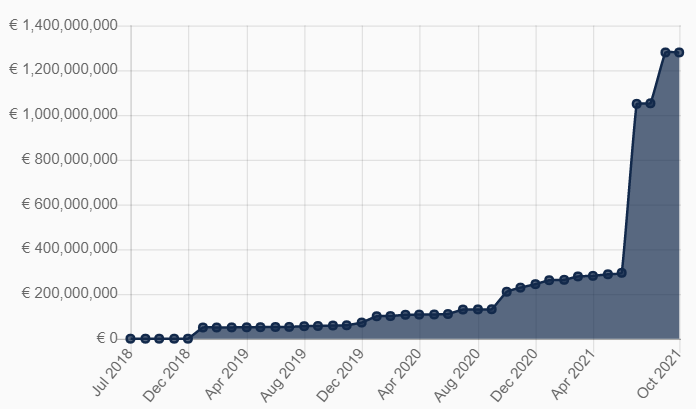
\includegraphics{EnforcementTracker_21-10-12.PNG}
		\caption{Enforcement activities \cite{EnforcementTracker}}
		\label{fig:enforcement_tracker}
	\end{figure}
	
	\section{Core Concepts}
	\startsection
	GDPR defines certain core concepts which are important for the further understanding of the regulation.\\
	\textbf{Personal data} is any information relating to an identified or identifieable natural person.
	There are three subtypes of interest to personal data. 
	First of, \textbf{sensible data} is defined as personal data that is revealing race, ethnic origin, political opinions, religious or philosophical beliefs, trade union membership, health, sex life and sexual orientation, genetic data or biometric data.
	Next, there is data relating to \textbf{criminal offences} and convictions.
	Finally, \textbf{health data} is personal data relating to physical or mental health of an individual, including the provision of health care services, which reveal information about his or her health status.\\
	\textbf{Pseudonymization} is the processing of personal data in such a manner that the personal data can no longer be attributed to a specific data subject without the use of additional information, provided that such is kept separately and is subject to technical and organisational measures to ensure that the personal data is not attributed to an identified or identifieable natural person.
	\textbf{Anonymization} eliminates personal data so that data subjects can no longer be identified. 
	Anonymized data is excluded from GDPR altogether because anonymized data is no longer personal data.
	\textbf{Data processing} means any operation or set of operations performed upon personal data or sets of personal data, whether or not by automated means, such as collection, recording, organisation, structuring, storage, adaptation or alternation, retrieval, consultation, use, disclosure by transmission, dissemination or otherwise making available, alignment or combination, restriction, erasure or destruction.
	\closesection

	\section{Data Processing Entities}
	\startsection
	GDPR defines different entities responsible for data processing, with various responsibilites.
	Namely there are the following:
	\begin{enumerate}[]
		\item The Data Controller (Art. 24 \cite{EUdataregulations2018})
		determines the purpose and means of the personal data processing.
		In general, controllers bear primary responsibility for ensuring that processing activities are compliant with the regulation.
		\item The Data Processor (Art. 28 \cite{EUdataregulations2018})
		acts on the conroller's behalf. 
		There is a binding written agreement between the two entities. 
		The controller must ensure the processor's compliance with GDPR.
		\item Joint Controller (Art. 26 \cite{EUdataregulations2018}) is a Data Controller, containing multiple entities.
		Given such a scenario, the different entities must have an agreement on their respective responsibilites.
	\end{enumerate}
	\closesection

	\section{Data Subject Rights}
	\startsection
	An identified or identifiable natural person, subject to its data being processed by a controller, is called a \textbf{data subject}.
	Each data subject has a set of rights under GDPR:
	\begin{enumerate}[]
		\item \textit{Right of access (Art. 15):} \\
		Controllers are obligated to provide all personal information being processed about a data subject upon request of the data subject.
		\item \textit{Right to rectification (Art. 16):} \\
		Controllers are obligated to rectify or complete wrong or incomplete data given a data subjects request to do so.
		\item \textit{Right to erasure (Art. 17):} \\
		One has the right to request deletion of one's personal data.
		Generally, given such a scenario, a controller must comply with such a request and furthermore inform all processors and joint controllers to eliminate the appropriate data as well.
		Furthermore the same procedure must be executed without being requested to do so under certain circumstances.
		For instance this applies, if the personal data is no longer necessary, the data subject has withdrawn consent or a deletion is mandatory due to other laws.
		Erasure of personal data is not lawful, if higher interests are diminished, controllers must namely not comply with such requests, when
		\begin{enumerate}
			\item the right of freedom of expression and information would be violated
			\item the controllers can not follow legal obligations without the personal data
			\item there is a public interest
			\item personal data is archived in public interest, used for scientific or historical research, or is used for statistical purposes
			\item the data is used to establish, exercise or defend of legal claims
		\end{enumerate}
		\item \textit{Right to restriction (Art. 18):} \\
		In general, a data subject has the right to restrict processing of its personal data.
		\item \textit{Right to data portability (Art. 20):} \\
		Controllers must provide collected data in machine and human readable format upon request, furthermore data subjects have the right to transfer the data to another controller.
		\item \textit{Right to object (Art. 21):} \\
		One can object to processing of one's personal data, then controllers are generally prohibited to process one's personal data.
		\item \textit{Right not to be subject to decisions based solely on automated processing which produces legal or similarly significant effects (Art. 22):} \\
		Controllers can not make decisions solely based on automatic processing, if the decisions produce a legal or similarly significant effect. 
		However necessary decision making for a controller to get into a contract with the data subject is explicitely excluded from this right.
	\end{enumerate}
	\closesection

	\section{Consent and Privacy Policy}
	\startsection
	Processors must issue a privacy policy.
	In the policy, basic information regarding processing activities must be provided in an easily understandable fashion.
	Given a data subject reads the policy, it should afterwards be well informed about the processing activities with its personal data.\\
	Controllers are prohibited to process personal data without the data subjects explicit consent.
	Therefore processors must acquire the data subjects consent, however this must be achieved in a way that:
	\begin{enumerate}[a)]
		\item Consent is freely given
		\item Consent is specific
		\item Data Subjects are informed on what they give consent for
		\item Consent is unambiguous indication of data subjects wishes
	\end{enumerate}
	In particular the data subject must have a legitimate choice, meaning it can not feel compelled to consent and there must not be negative consequences if consent is not given.
	This implies that consent can not be bundled with acceptance of other terms and conditions, 
	it can not be tied to the provision of a contract or service, if the processing is not strictly neccessary for the perfomance of such a contract or service and
	data subject should be able to selectively consent to separate processing activities - i.e. a data subject should be able to consent to processing of performance data but reject processing of marketing data.\\
	Due to the above regulations, contollers must manage to demonstrate data subject's consent and ensure potential withdrawal.
	Therefore controllers should keep clear records of what a person has consented to, when and how consent was obtained in order to be able to give evidence of consent if challenged. 
	In particular, controllers should store:
	\begin{itemize}
		\item Date of consent
		\item Method of consent
		\item Who obtained consent
		\item What information was provided to the person consenting
	\end{itemize}
	The data subject should also be able to revoke its given consent at any time which should be as easy as to give consent. When the consent is rescinded the data must be deleted immediately and the further processing of it is prohibited but the former processed data can still be used.
	\closesection

	\section{Sanctions}
	\startsection
	GDPR imposes hefty fines for non compliance with the regulation.
	It differs between two groups of violations: Violations with respect to record-keeping, security, breach notifications, and privacy impact assassments and violations with respect to having a legal justification for processing, complying with the rights of data subjects, and cross-border data transfers.
	The first group is subject to a maximum penalty of the highest of 10 million Euro or 2 \% of the entity's global revenue and the second group a maximum penalty of the highest of 20 million Euro or 4 \% of the entity's global revenue, respectively.
	\closesection
	
	
	\chapter{Crowd-Sourcing Methods}
	Before concerns regarding privacy of crowd-sourcing methods can be addressed, it is imperative to list a subset of the options that are in use today.
	
	\section[Amsterdam]{Amsterdam \cite{SmartCityAmsterdam}} \label{Amsterdam}
	\startsection
		Amsterdam was on of the first European cities to adopt the concept of smart cities launching a holistic strategy in 2009. The government realized early on that there exists 4 key groups, namely governement, businesses, universities and research institutions, and citizens, to the creation of a truly smart city. Beneficial to enabling communication, coordination, and collaboration the government of Amsterdam created a Smart City online platform which is used by an organized partnership of twelve public, private and university/research partners such creating a sort of marketplace where ideas and project initiators can be matched with potential developers and implementation partners.
		\paragraph{Enabling Initiatives} \hfill \\
		Several companies established a network of \href{https://www.yenlo.com/blogs/ibeacon-testing-ground-first-lora-network/}{iBeacons}, which are small devices that can connect to smartphones, wearables and other devices via Bluetooth in order to enabling apps to receive much more specific, location-based data under a collaboration named "Internet of Things Living Lab". Along 3400 meters these beacons are positioned and can communicate with other devices up to 3 kilometers away, thus being able to send data to a cloud in order to be used for smart city development.
		\paragraph{Social Initiatives} \hfill \\
		The smartphone application \href{http://www.urbyapp.com/}{Urby} is used such that based on location and interests of the user local events and activities are suggested hence saving time for the user which would be spent in order to find those but hence indirectly promoting the businesses hosting the events and activities.
		\paragraph{Infrastructure Initiatives \cite{SmartCityAmsterdamYT}} \hfill \\
		Amsterdam is setting up smart lighting areas throughout the city, so the municipality can control the intensity of the lighting posts depending on where they are located and whether the traffic volume does have a great need for it. With movement sensors it is ensured that the lights reach the maximum brightness if citizen or vehicles pass them and the minimum when ther is noone around. It is also possible for police departments and traffic offices to bring the intensity of the light post to the highest point in case of emergencies, like evacuation. To further enhance smart energy usage electric car loading stations are using so called "Smart Charging" by either delaying at what time the loading station starts to load the vehicle or reducing the output according to the current grid utilization.
		\paragraph{Mobility Initiatives} \hfill \label{AmsterdamMobilityInitiatives} \\
		Concerning traffic congestion Amsterdam and other cities found out that about a third of all city traffic is created by people in search of a parking spot. In pursuance to remove this third from the streets and help the drivers to find the required spot faster, sensors were embedded in parking spaces, which communicate with a cloud so end-users can track down the nearest available space via app. As statistics have shown this led to a reduction in the average time to find a parking spot of 43\%. In order to further reduce traffic the smartphone app Toogethr makes carpooling easier by matching passengers with potential drivers based on the location of their home and employment and the working hours and thus leading to a reduction in pollution and fuel usage.
		\subsection[Schoonschip]{\href{https://schoonschipamsterdam.org/en/}{Schoonschip}} \label{Schoonschipp}
		\startsubsection
			Located in the Johan van Hasseltkanaal, situated in the North of Amsterdam, Schoonschip is a ecologically and socially sustainable, floating neighborhood, housing 47 households on 30 residential units (arks). With heat pumps that extract warmth from the water in the canal (aquathermie) and solar panels on top of each house the residential area can be self sufficient in the summer. All of the individual systems of each residential unit is connected with one "My-Power-Grid" energy grid system which uses realtime data in order to decide, using additional wheather and solar information, on what to do with the enrgy, in order to optimise each house's energy production. Also it can conclude whether it is best to charge or discharge batteries or storing energy as heat in the heat pumps. Because of the need of the information of what the energy consumption in Schoonschip is at any time the data is shared for everyone to see (https://schoonschipamsterdam.org/en/).
		\closesection
	\closesection
	
	\section[Boston]{Boston \cite{SmartCityBoston}}
	\startsection
		Just like Amsterdam, Boston's then Mayor Thomas Michael Menino, threw the hat into the ring of innovation by launching experimental smart initiatives in the year 2010. In his vision, Boston should be a host for innovations, rather than depend on the ones thought up and developed silently in universities and research firms. This realization of this vision has lead to the creation of numerous jobs and companies, while also marking Boston's Seaport as the Innovation District in the eyes of Mayor Menino for years to come.\\
		A selection of these initiatives will be presented in the following sections, as they focus heavily on crowd-sourcing in respect to smart urban participatory applications and smart transportation.
		\subsection[BOS:311]{\href{https://311.boston.gov/}{BOS:311}}
		\startsubsection
		The application called "BOS:311" "deputizes" the citizens of Boston and allows them to report various issues found on the streets like potholes, illegal graffiti and so on. The users can report an issue by selecting out of a number of services, like "Litter", which best corresponds to the found issue, add the location over Google Maps, take a photo, and add a description. Additionally the user can state if he wishes to share the report with the public, and he can also record his name and contact information, thought these will not be publicized. 
		\closesection		
		\subsection[Where's my School bus?]{\href{https://schoolbus.bostonpublicschools.org//}{Where's my School bus?}}
		\startsubsection
		Another application for parents is "Where's my School bus?". The application allows the parents to track their children's school bus in real-time by logging into the application using their child's information and student number. This of course implies that all of Boston's school buses are fitted with tracking functionality.
		\closesection		
		\subsection[Waze]{Waze \cite{InformationSuperhighway}}
		\startsubsection
			Waze is an application that specialises on route planning and traffic avoidance.
	Bostons traffic management department partnered with Waze to combat the cities traffic issues. Waze delivers hereby the data of driving app users to the Boston traffic engineers which then adjust the cities traffic signals. The traffic department also sends back this updated information in addition with future planned adjustments to Waze in turn.
		\closesection
		\subsection[Street Bump]{Street Bump \cite{EGG17}}
		\startsubsection
			In the same manner as the Waze partnership, Boston used the Street Bump application for combating and mapping bumpy roads and potholes. This allowed the city to repair the worst cases of potholes and, as an unexpected side benefit, sunken manhole covers (\href{http://www.streetbump.org/about}{streetbump.org/about}) \cite{BostonStreetBumpTOS}. \\
			Citizens of Boston can download Street Bump from the App Store on their smartphones. Afterwards they are able to record their car trips and send the record to Boston itself. The potholes and street bumps can be recognized on the city maps by using the phones accelerometer and GPS. The city of Boston only inspect such roadway problems if there are multiple hits from large volumes of data, this provides some form of protection against false positives.\\
			Street bumps terms and conditions state that the following data is collected and how it is used:\\
			Major changes in vertical accelerations are combined with GPS locations, a trip consists of all such bumps. Street bump does not collect the route data itself. 
			All bumps are consumed by a clustering algorithm to discover the likelihood of road issues. To focus only on this five more data points are collected, namely date and time of the bump, the GPS accuracy, speed of the car, the course, in essence a scale from 0-360, where 0 is north, the distance travelled, and phone information, like a unique ID, operating system, model and so on.
			Optional information is the contact information of the user which is not collected by default. If the user chooses to then some personal information like name or email will be linked to the unique ID.\\
			Further data that is collected to enhance Street Bump are the aggregated use statistics, invalid bumps with added reason why it is valid and stripped location information, failed upload information, and failed trip information\\
			The following entities can see the data:
			All data is viewable by the city of Boston and its partners. The participating municipalities and other entities can see the identified obstacles and the composite bump data.
			Neither the contact information nor user specific bump data is shared with these entities.
			The public can see the obstacles and composite bumps on 'streetbump.org'. The individual bumps will only have the date, location and accelerometer readings. If the specific bump is not part of the obstacle it will not appear.  The site will also display a map of recent bumps. The map is hereby centered on a collection of bumps and not necessarily where the bump or trip was. Users are able to choose if their bump data appears publicly.\\
			In the international usage, the user gives permission to store and process their data in any countries where Street Bump facilities exist. This includes the transfer of personal information. If the user disagrees with the policy then he should not use Street Bump.
		\closesection	
		\subsection[Yelp]{Yelp \cite{YelpBoston}}
		\startsubsection
			A third partnership performed by Boston, was with Yelp and economists from Harvard to tackle the issue of health inspections at restaurants b using predictive algorithms and experience from health inspectors.
			Instead of random inspections, information from recent customer reviews on Yelp and historical patterns are taken into account to better target the restaurants under suspicion of health code violations. The increase in found violations has been estimated to be around 30\%-50\% \cite{BSL16} \cite{Gla16}.
		\closesection
	\closesection
	
	\section{New York City}
	\startsection
		\subsection{Building Inspection}
		\startsubsection
			New Yorks department of buildings had too few inspectors to cover all complaints about illegal conversions of apartments in a sensible manner in the year 2011. This is a complicated situation as such conversions of living space increases the risk fire hazards among other dangers. As an answer, a team led by Michael Flowers has used predictive analytics have been used to prioritize the complaints by also incorporation the experience of senior inspectors \cite{BeyondOpenData}.\\
			Thanks to this new prioritization, the false positives of the complaints have been drastically reduced, which increased the ration of resulting vacation orders from 13\% to 70\% \cite{PredictiveDataAnalytics}.
			Additionally, this has positively influenced the incidents of deaths due to fire incidents as mentioned by the city \cite{BigDataBigApple} \cite{FDNY}.
		\closesection
		\subsection[Wiki Survey]{Wiki Survey \cite{BitbyBit}}
		\startsubsection
			Wiki surveys differ from normal surveys in the way that the answers do not have a finite number, but are in an open form, so that each participant can give answers outside of the expected scope. These outside answers are also exactly the reason to perform such a survey as it allows for new perspectives to be considered. For example New York City performed a wiki survey in 2010 on its sustainability plans, and eight of the top ten ideas where generated from the survey takers instead of being in the set of seed answers.
		\closesection
	\closesection
	
	\section[Palo Alto]{Palo Alto \cite{SmartCityPaloAlto}}
	\startsection
		In 2014 the municipality of Palo Alto, Santa Clara County, California, ran an app creating challenge. In this participants were asked to develop apps addressing the solution of a problem or providing a service important to the community. From this challenge various apps emerged, like the AdoptMe! app which is focussing on sharing the stories and ultimately finding a home for animals that are kept in shelters or in foster care, or the Play Palo Alto app in which challenges and missions can be completed by both visitors and residents in order to earn points which can then be redeemed for coupons at local businesses and restaurants. Also a result of this competition was a guidebook co-authored by the city's CIO called "The Apps Challenge Playbook" \cite{AppsChallengePlaybook} on how to run a successful Apps Challenge so other cities can carry out these events as well. Since then Palo Alto introduced many different Smart City Initiatives in order to solve the problems of its citizen.
		\paragraph{Infrastructure Initiatives} \hfill \\
		Together with the local institution Stanford University the city places sensors, especially in Palo Alto's retail district, to track air quality indicators. A similar approach is made to monitor the water use which can not only suggest ideas for water-saving measures but also can work as an early warning system for leakages. Similar to Amsterdam (Section \ref{Amsterdam}) a smart lighting and electricity grid shall be installed in the near future.
		\paragraph{Municipal Initiatives} \hfill \\
		In order to increase the response time of government services and simplify the access to it for its citizens some fields of operation transitioned to the digital world, i.e. a chatbot on Facebook that can answer simple queries for frequently asked questions or apps for emergency situation preparations and planning tips. Additionally an app was developed with which citizens can directly report different civic grievances like littering and certain types of crimes and even follow up the city's response. Furthermore Palo Alto introduced its citizens to the \href{https://coolblock.org/}{Cool Block Project} which focuses on giving solutions in specific areas like watching water use, preparing for bad situations, and reducing the block's carbon footprint.	
		\paragraph{Mobility Initiatives} \hfill \\
		As seen in Amsterdam also Palo Alto (Paragraph \ref{AmsterdamMobilityInitiatives}) uses the same approach in order to oppose traffic congestion by letting the drivers know where the nearest parking spot is. Another target is the broader control of traffic flow. By connecting the traffic lights into a single, large network and using sensors so dynamic and remote signalling is made possiblethe traffic safety can be improved and the response time for emergency services can be reduced. Through collecting statistics on different traffic types and flow direction smart city planning is also enabled and new smart city mobility solutions can be created.
	\closesection
	
	\section{Nokia}
	\startsection
		\subsection[Nokia AVA]{Nokia AVA \cite{NokiaAVACrowdAnalytics}}
		\startsubsection
			The company Nokia developed a series of analytical services and AI products for other communication service providers under the name Nokia AVA, which stands for Analytics, Virtualisation, and Automation. Nokia AVA aims to analyse the network and customer data of the providers for improvements in customer care and engagement, their service operations and how to further optimize the network itself.
			To better showcase the benefits of their product, Nokia has made three case studies available on their homepage, namely for Vodafone, POST Luxembourg and China Mobile, which will be presented and exemplified in the following sections.
			\subsubsection{Vodafone Anomaly Detection in Italy}
				Vodafone decide to launch an anomaly detection application in Italy in partnership with Nokia for their network planning and optimisation. Vodafone has provided their own network data, while Nokia provided the applications and models for successful implementation. Vodafone noted an increase in operational efficiency of 25-30\% and plans to deploy to other countries.	
			\subsubsection{POST Luxembourg}
				POST Luxembourg wanted to reduce operational costs and increase customer satisfaction by diagnosing issues on the network through AI application and increasing the efficiency of their field technicians.
			For this POST Luxembourg used Nokia's home and access insight solution, which is aimed at analysing and resolving network issues. The usage resulted in a 95\% correct or helpful diagnosis received by their field staff.
			\subsubsection{China Mobile}
				China Mobile was concerned with increased energy usage across their network especially due to rolling out 5G, and searched for an intelligent energy management system that does not impact customer experience.
				A solution has been found in the form of Nokia AVA for Energy Efficiency, and resulted in a reduction of short-term energy use of 5\%, made future reduction of 20\% possible, reduced air conditioning energy usage by 74\%, generally balanced performance requirements with energy saving, and maintained the network performance successfully.
		\closesection	
		\subsection[StarHub]{StarHub \cite{StarhubNokia}}
		\startsubsection
			A further partnership between Nokia and the singaporean  based communication provider StarHub has been created with the goal of 'effective advertising'. This means that marketers can for example plan their future business locations and placements of advertisements due to gained insights from consumer travel patterns. StarHub hereby plans to use Nokia AVA and other capabilities from Nokia. 
		\closesection
		\subsection{General Assumptions about Data and Privacy}
		\startsubsection
		Nokia and its partners have not revealed how exactly privacy is handled in their projects, in addition to how data is analysed, processed or transformed. Assumptions can be made that GPS coordinates of users are involved in some form for the effective advertisement and the project in China, at the very least. It would be reasonable to assume that all partners of Nokia have some measurements in place to protect their users privacy in addition to protocols for handling successful attacks, because, as communication providers, they remain a lucrative target for malicious entities.
		\closesection		
	\closesection
	
	\sectionmark{Nokia AVA}	
	\section[Test Case Studies and Modeling]{Test Case Studies and Modeling \cite{CrowdSourcing}}
	\startsection
		Test case studies have been performed with current examples of crowd-sourcing like Street Bump to show how certain sectors can profit from crowd-sourcing methods. For example in the dimension of transportation, it would be possible to dynamically allocate parking spaces with crowd-sourcing or similar to previous examples the app CycleAtlanta that records bycicle trips and sends the data to the city planners of Atlanta. In the sector of education, sites like Khan Academy or Un-Academy allow for educators to teach to groups of all ages. Other education based sites that use crowd-sourced of users are for example sites like Wikipedia, Quora or StackExchange. In the sector of healthcare, there exist websites where users can share their patient experiences and receive information about sickness and diseases.
	%There are more examples though I think this is ok for now.
	\closesection

	\section[Mobile Crowd-Sourcing]{Mobile Crowd-Sourcing \cite{MobileCrowdSourcing}}
	\startsection
		Mobile crowd-sourcing puts the various sensors and systems of mobile devices in focus. As in previous sections seen this allows for optimal data gathering in domains like monitoring of traffic for example.
		The most common architecture of mobile crowd-sourcing is made up of three entities, namely the working crowd, service providers, and end-users. The workers perform tasks received by the service providers and return the results. Service providers receive requests from end-users and divide them into smaller subtasks for its workers to perform before sending finished tasks back to its end-users. The service providers also collects and processes data, and is also responsible for evaluating its participants if needed. The end-users can send request to the providers and also evaluate the results later.\\
		To better decide which workers are suited for which tasks, a task recommendation and allocation system can be used that, for example, collects and analyses the participants context information, like location, usage of the platform, previous work evaluation, and other data points. Such a system can improve the efficiency of task assignment in the context of throughput and quality.
	% There is more information about MCS, should this also be added?
	% The paper also states some possible further applications of MCS
		\subsection{Privacy control, Concerns, and Threats of Mobile Crowd-Sourcing} \label{PrivacyMCS}
		\startsubsection
			Privacy concerns arise due to the need of environmental data of the participants for the task recommendation system. If the system does not have any safety measures an attack can breach the privacy of the platform. \\
			The human involvement, task crowd-sourcing itself, and the dynamic topology can make privacy protection difficult.
			For example the sensing worker can collect and send data pertaining to his location, which can reveal his movement, or could also contain identifying or private information that could be collected by malicious entities. Additionally on part of the service provider, the difficulty for privacy security increases especially if the outsourced tasks contain sensitive information to complete the task. Another challenge for privacy protection can be the changing topology of the network, due to joining, leaving and movement of workers, and weaken the possible protection against outside attackers \cite{SecPriMobCSM}.\\
			Furthermore there exists privacy threats that can be identified as privacy threats from data and privacy threats from tasks itself. As mentioned before, the privacy of the sensed data consists of the danger that collected data contains identifying information, or more general information that can leak privacy, be it environmental, locational, routine, and so on. Similarly, the privacy of computing inputs considers the sensitive data that is enclosed in the tasks itself, which may leak the data of contributors/workers, data owners and other related people. This encapsulated data could consist for example as personal health information, business reports, among other information. Finally the privacy of computing results can occur if the task results itself contain sensitive information that should not leak to the worker or the service provider, and only remain in the hands of the end-user. Evidently, setting up systems that accomplish such conditions can be difficult.\\
			Further threats to privacy could be identified originating from the tasks, in the form of task privacy of end users, and task privacy of participants. Focused on the end user privacy, it can occur that the content of the stated tasks can reveal information of the end user to the service provider, for example if the task pertains to traffic information on the street, it could be inferred that the end user is in possession of a car. For the privacy of the participants it is important that the tasks itself do not leak information about the participants/workers. Again the example of worker location tracking can be mentioned.\\
			Additional privacy concerns have been identified in \cite{PrivacyAwareMCS}. The concern of disclosed user identity states that many mobile crowdsourcing systems collect profile informations of their participants/workers, like name, password, email address and so on. If this data could be breached and retrieved by attackers, then it could have far reaching consequences to the participant. Again mentioned has been the disclosure of user location and activities, just as in the previous paragraph, but with the added idea that the worker/participant may be aware that his activity and location may be monitored but not to which degree, due to ignorance. A second thought goes to the requirement for users that want to share data about general locations and activity but not for sensitive places. The lack of user privacy awareness, as mentioned before, is the idea that the user does not have the knowledge of how the data will be used and in how much privacy risk he is, and therefore has no choice but to trust the application.\\
			Indeed the inability to know or deduce the usage of the gathered data for the common man itself brings further vulnerability. It could occur that the gathered data itself is relatively privately secure but if businesses combine this data with further information gathered from other sources could lead to insights about private information of the users. Lastly, one must consider the usage of mobile devices itself due to increased vulnerability to attacks and security breaches. Mobile devices mostly have limited computational resources to incorporate certain cryptographic protections.\\
			The publication "A Survey on Security, Privacy and Trust in Mobile Crowdsourcing" explores various schemes for mobile crowd-sourcing networks. The evaluation is based upon the fulfillment of requirements in regard to trust, privacy and security of the schemes. Especially for guaranteeing privacy, differentially privatize the sensed data and addition of noise, homomorphic encryption for the personal information, or grouping areas of workers together for further generalization, or data aggregation have been proposed in some schemes for example. Nonetheless, it is difficult to develop a scheme for mobile crowdsourcing that fulfils all three requirements for trust, security and privacy \cite{SecPriTrustMCS}.
		\closesection
	\closesection


	%\chapter{Considerations in Designing Crowd-Sourcing Methods}
	\chapter{Results}
	In the following chapter the currently used crowd-sourcing methods are evaluated and possible design principles and guidelines are introduced.
	
	\section{Today's Crowd-Sourcing Methods and GDPR} \label{juxtaposition}
	\startsection
		Generally, today's crowd-sourcing methods are GDPR-conform and can still be carried out as before. \\
		However, there are some critical and tricky points that need to be considered when a government or service provider wants to use a certain crowd-sourcing method. \\
		First of all, it must be ensured the "Right to Restriction" and the "Right to Object" must be respected, as there must be an option to prevent the data processing of a certain individual. For example due to the high-quality cameras that are available for tracking purposes, such as traffic flow surveillance, public spaces which are not part of the actual video scanning can be intruded and people which are staying in these spaces can be recognized due to the progress in facial recognition algorithms. \\
		Other precarious rights are the "Right to Access" and the "Right to Data Portability" such that apps, which were not developed by the government but by individuals, do not grant easy access to the data which were gathered and therefore are not in compliance with GDPR. Additionally, such cases can be very difficult to enforce if the service provider's location is either outside of the European Union or can not be clearly identified. \\
		For most of the crowd-sourcing methods the "Right to Erasure" can be neglected, because most of these are used to achieve a goal of "public interest" therefore nullifying the associated paragraph.
	\closesection
	
	\section{Guidelines and Design Principles}
	\startsection
		The very first thing to mention is that GDPR is only considering personal data, hence anonymized data is out of scope regarding the regulations. Therefore, when using data in use-cases where it does not matter who this data belongs to, it should be anonymized in order to rule out possible conflicts with GDPR. \\
		A very important point when developing crowd-sourcing methods is the handling of consent. It must be given before gathering any data of the data subject, which also must be fully informed of what data is collected and for what purposes. It is not allowed to inline the consent giving in the terms of condition but it must be a separate paragraph which can be individually approven or neglected. The choice must not have any negative consequences as loss of services for instance. If the consent consists of several parts, like the data that is collected, it should be made adjustable such that a full control of what is congregated is given to the user. If a user does revoke his/her given consent the data collection must stop immediately, the already gathered data must be deleted and processing it is prohibited. However already processed data can still be used for information seeking. \\
		In order to directly comply with the rights of a data subject stated in GDPR the following guidelines must be considered:
		\begin{enumerate}[(a)]
			\item All data that is gathered and processed must be accessible by the user and can be handed out when requested.
			\item Restriction and Objection of data processing must be made possible.
			\item If the crowd-sourcing method is not used to achieve a goal of public interest the data must be deleted on request and its processing must be prohibited.
		\end{enumerate}
		Following are some design principles and solutions for certain conflicts that were stated before: \\	
		As mentioned in section \ref{juxtaposition} when using cameras in order to surveil certain places, like traffic flow observations, public spaces should be intruded as little as possible by either replacing or reinstalling the camera or by using a blur zone filter, as described in the paper "GDPR Compliance in Video Surveillance and Video Processing Application" \cite{GDPRandSurveillanceCameras}, in order to make some parts of the field of view unidentifiable. \\
		The gathering of GPS data in realtime can be critical as already stated in the subsection \ref{PrivacyMCS}. If the realtime aspect of the gathering is not of much use, the approach of Apple presented in their paper "Learning with Privacy at Scale" \cite{PrivacyApple} can be used with which the data is sent independent from the timeframe the data was generated. The data is stored on the device which created it and at an arbitrary point in time it is actually sent to the provider of the application or service that wants to use this data, therefore detaching the realtime aspect and make it somewhat impossible to trace back the point in time of when the data was produced. \\
		For services and application where realtime is also a relevant information to be processed as the energy and water consumption in smart homes, for example in the Schoonschipp project in Amsterdam (subsection \ref{Schoonschipp}), whose smart grid system relies on that data, the General Data Protection Regulation can be a really hard to implement directive, because the inhabitants are "transparent human beings" as the data from the homes is publicly known. Therefore the consent part of GDPR is significant such that the inhabitant are well informed and authorize the service provider to use that data, hence making GDPR somewhat redundant and unnecessary in such cases.
	\closesection
	
	\hfill \\
	\noindent The idea of GDPR is to give users back the power over their own information and data and decide when it is used. Also because the use of data has become highly technical, obscure and unpredictable the concepts of consent which are the underlying base of the privacy rights are not meaningful as tracking the data in the world wide web and other services is very difficult. Another idea emerged in 2018 in the paper "A Blueprint for a Better Digital Society" by Jaron Lanier and E. Glen Weyl of "Data Dignity":
	
	\section[Data Dignity]{Data Dignity \cite{LanierWeylBlueprint}}
	\startsection
		In todays' world few gigantic tech firms like Alphabet or Facebook have become so powerful that they are able to use their platforms, like YouTube, to control what content will be consumed or who does get paid for the generation of the media/data. Lanier and Weyl compare this to communism in which a central planner makes analogous decisions. An idea to oppose this scheme is to create a business model in which data creators will directly trade their generated data to tech firms and other services that want to use this data for training machine learning algorithms or to draw conclusions for new advertisement campaigns, the so called "Data Dignity". \\
		The idea behind "Data Dignity" is to create a coherent marketplace for people's data in which people are getting paid for the data they generate and have to pay if they want to use services that need this data. A benefit of this is that platforms will receive higher-quality data and therefore being able to create higher-quality services with which a greater revenue can be achieved. \\
		In order to enforce data dignity Lanier and Weyl suggest the use of "Mediators of Individual Data", so called MIDs, because tech firms or individuals alone would not be able to make this kind of change as for tech giants too many conflicts of interests do exists and the complexity of the digital economy does not allow the in detail regulation. These MIDs are intermediary groups which will negotiate with service providers that need data about the value of data and the wages and data royalties of them and will perform payment duties, so the individual that generated the data gets paid acoordingly. They are representatives of a group of people, like corporations or labor and consumer unions, which will promote its own standards and qualities. MIDs can be really different from another based on the members that they represent or which interests are of the most value for them. It is also possible that for some of the MIDs not everyone is allowed to or it is really hard to join them, based on the data they are handling. However, all of the MIDs should in some way implement the following eight principles:
		\begin{enumerate}[(i)]
			\item \textit{Fiduciary Duty} \\
			An MID should be a trustee for individuals that create data. The data from the user's should therefore be measured in a legal, economic, and structural sense.
			\item \textit{Quality Standards} \\
			Each MID can individually define quality standards, enforce and foster them in regards to decency, accountability, and acknowledged achievements.
			\item \textit{Inalienable Provenance} \\
			An MID should handle the buy- and sell-procedure of data to service provider, but should also ensure that the data is only used for the specific processes and not be either permanently sold or the use is alienated beyond recognition.
			\item \textit{Benefit Sharing} \\
			Each MID should ensure that most of the benefit (approximately 70\%) is given back to the creators. This may need a regulatory layer in the whole system in order to guarantee this.
			\item \textit{Competence and Professionalism} \\
			An MID should have an expertized management such that it can be entrusted by the data creators to competently and in a position of parity negotiate with data customers and service providers.
			\item \textit{Biological Realism} \\
			A user should not be compensated based on quantitative, ideal measures but on the needs of the user which can change with age and time. An MID should encourage its data creators to build up a "portfolio" of data royalties over their life time in order to gain some revenue after retirement.
			\item \textit{Cognitive Realism} \\
			An MID should be easy to understand and not come with long terms and conditions or complex consent giving processes, like it is the case in today's world.
			\item \textit{Longevity} \\
			An MID should not be a short-lived venture, but a long-lasting, intergenerational intermediary for wisdom and data. Also MIDs should create a relationships among themselves, like MIDs for nurses with MIDs for biological scientists, in order to create a network of exchange and research.
		\end{enumerate}
		This idea is much more systemic and future oriented than the introduction of privacy regulations in respect to not being able to prevent even more innovative privacy regulations by directly involving individuals in this topic so they realize the benefits of reasonable limitations on what efforts are demanded of them, fair compensation for what information they reveal about themselves among other abilities. Weyl and Lanier abstractly call this "the right to be left alone".
	\closesection
	
	\chapter{Conclusion}
	
	\newpage
	\addcontentsline{toc}{chapter}{Bibliography}
	\printbibliography
\end{document}
